\newpage
\section{評価実験}
\subsection{収縮率}
作製した内径5 mm,3 mmの人工筋肉の収縮率の測定を行った.
収縮率は
$$\frac{(収縮後の長さ)-(収縮前の長さ)}{収縮後の長さ}\times 100\\$$
で計算を行った.
図\ref{fig:oiru}に測定するにああたって必要な部品を示す.必要な物品は以下の通りである.
\begin{itemize}
    \item 作製した人工筋肉(内径5 mm,3 mm)
    \item オイルレス エアーコンプレッサー 39 L
    \item フィルターレギュレーター AW30-02BG
\end{itemize}
\begin{figure}[h]
    \centering  % 図全体を中央に配置
    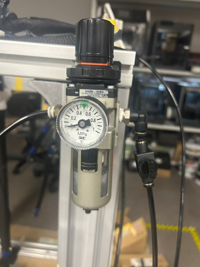
\includegraphics[scale=0.5]{pic/oiru.PNG}
    \caption{使用方法}
    \label{fig:oiru}
  \end{figure}
測定方法を以下に示す.
\begin{enumerate}
    \item 膨張する前の人工筋肉の長さを測定する
    \item 人工筋肉をエアーコンプレッサーに取り付ける
    \item 人工筋肉の膨張を確認しながらノズルを回し,破裂しないギリギリまで膨張させる
    \item 膨張した状態を保ちその状態を測定する
\end{enumerate}
\subsubsection{内径5 mmの測定}
図\ref{fig:zzA}に今回作製した内径5 mmの人工筋肉を示す.
上記の方法で空圧を印加すると0.02Mpaが膨張の最大となった.
空圧印加前の長さは75 mm,空圧印加後の長さは68 mmで収縮率を求める式に代入すると
$$\frac{(68 mm)-(75 mm)}{68 mm}\times 100\\$$
となり収縮率が10.7 \%となることが確認できた.
\begin{figure}[ht]
    %
    \begin{minipage}{0.49\columnwidth}
      \vspace{4mm}
      \centering
      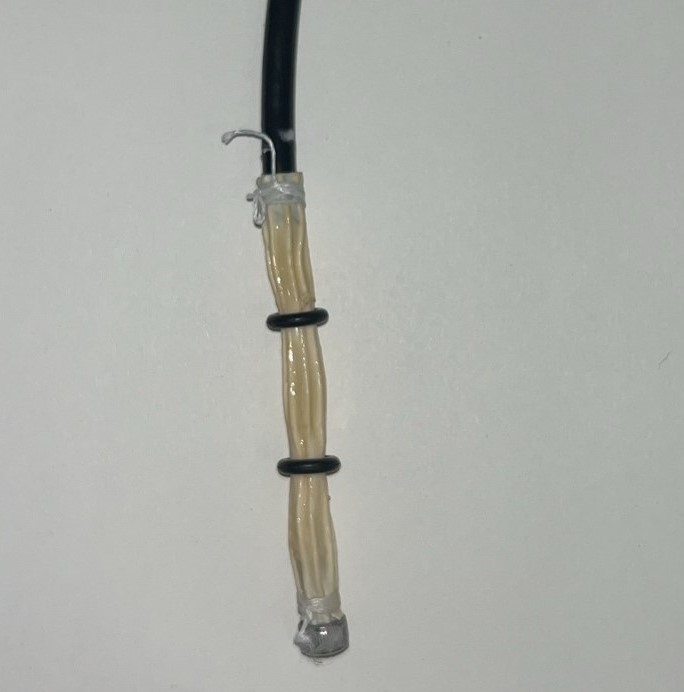
\includegraphics[scale=0.3]{pic/D.jpg}
   
      \subcaption{空圧印加前}
      \label{fig:inn}
    \end{minipage}
    %
    \begin{minipage}{0.49\columnwidth}
      \vspace{4mm}
      \centering
      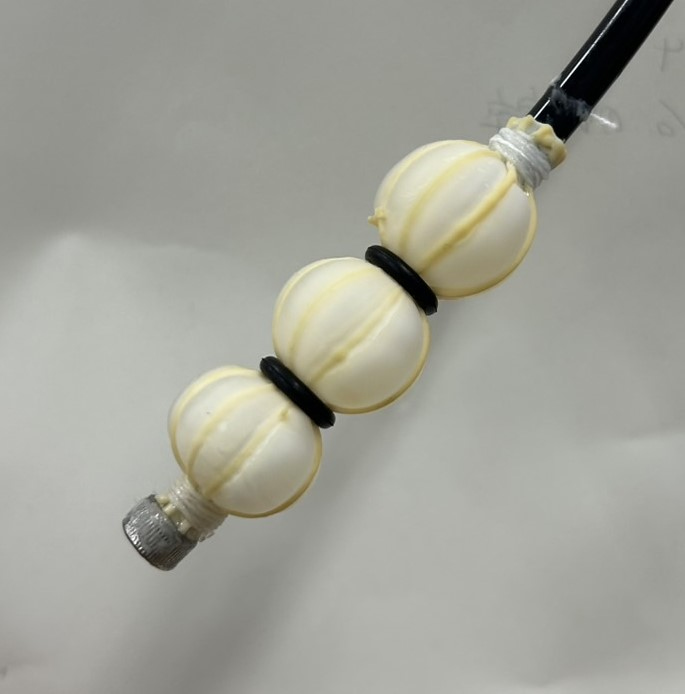
\includegraphics[scale=0.3]{pic/E.jpg}
      \subcaption{空圧印加後}
      \label{fig:ato}
    \end{minipage}
    %
    \caption{内径5 mmの人工筋肉}
    \label{fig:zzA}
  \end{figure}.
\subsubsection{内径3 mmの測定}
図\ref{fig:zA}に今回作製した内径3 mmの人工筋肉を示す.
上記の方法で空圧を印加すると0.06Mpaが膨張の最大となった.
空圧印加前の長さは54 mm,空圧印加後の長さは49 mmで収縮率を求める式に代入すると
$$\frac{(49 mm)-(54 mm)}{49 mm}\times 100\\$$
となり収縮率が9.3 \%となることが確認できた.
\begin{figure}[h]
    %
    \begin{minipage}{0.49\columnwidth}
      \vspace{4mm}
      \centering
      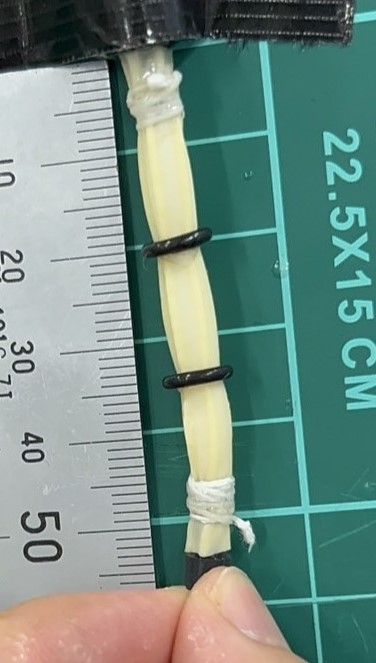
\includegraphics[scale=0.3]{pic/M.jpg}
    
      \subcaption{空圧印加前}

    \end{minipage}
    %
    \begin{minipage}{0.49\columnwidth}
      \vspace{4mm}
      \centering
      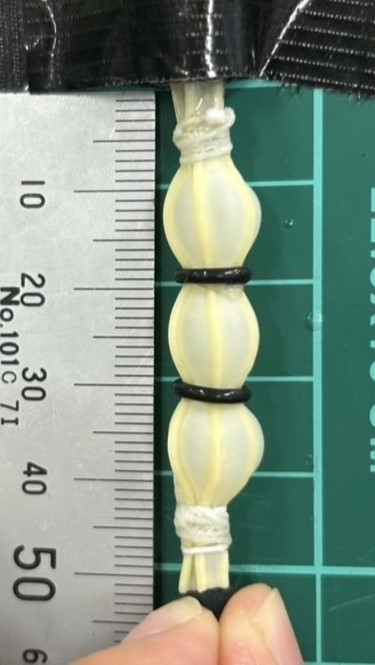
\includegraphics[scale=0.3]{pic/L.jpg}
      \subcaption{空圧印加後}
      
    \end{minipage}
    %
    \caption{内径3 mmの人工筋肉}
    \label{fig:zA}
  \end{figure}.
\subsection{発揮張力}


